\section{Linked Environments for Atmospheric Discovery}
\label{se:lead}

\acrfull{lead} \cite{Droegemeier2005Service-orientedWeather} addresses the fundamental research challenges needed to create an integrated and scalable framework for adaptive analysis and prediction of the atmosphere. The weather forecasting researchers require many computer resources to predict and analyze weather models in the mesoscale with less time. Rather than each researcher run and handle their computer resources for the weather experiments, LEAD provides a shared pool of resources. Then the researchers can use the resource pool to run their experiment in shorter amounts of time and a more massive scale. At the time, some researchers are developing their experiment forecasting flows, they are not using the resources, and other researchers can run their forecasting flows using available resources. The foundation of the LEAD system is to create a dynamic workflow orchestration and data management in a web services framework \cite{Droegemeier2005Service-orientedWeather}.

LEAD's complex range of services, applications, interfaces, and IT resources, local and external networks, and storage is compiled by users in workflows to study mesoscale incremental manner \cite{Droegemeier2005Service-orientedWeather}. As it follows the SOA, all the features are implemented as independent services. The above implementation enables LEAD to scale up each service as required and update each service without affecting other services. New models that are required for implementing a new forecast flow also have to be implemented as a service and then integrate into the system.

\cref{fi:lead_system} shows the key capabilities of the LEAD system. The top layer of the LEAD enables users to search and acquire information, simulate and predict weather conditions using digital atmospheric models, assimilate, analyze, use and visualize data and output of models.

\begin{figure}[htp]
    \centering
    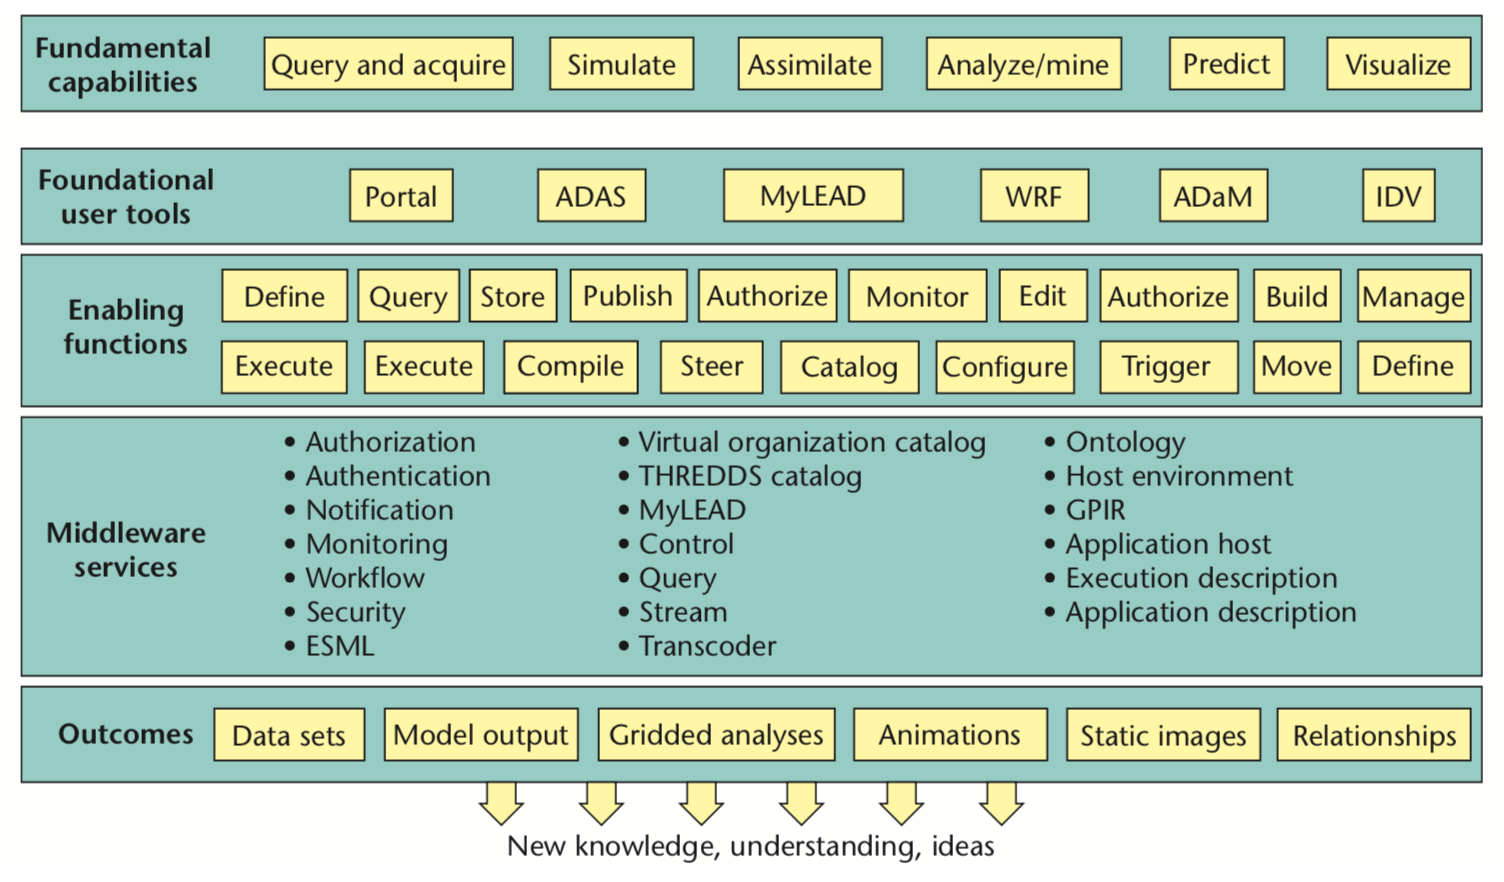
\includegraphics[width=1.0\textwidth]{lit/lead/LEAD-system-Fundamental-capabilities-familiar-to-meteorologists-are-shown-in-the-top_W640.png}
    \caption[Layered architecture of LEAD]{Layered architecture of LEAD \cite{Droegemeier2005Service-orientedWeather}.}
    \label{fi:lead_system}
\end{figure}

The second layer contains fundamental tools such as the following to help to link services together \cite{Droegemeier2005Service-orientedWeather}:
\begin{itemize}
    \item The users interact with LEAD via a web portal
    \item Data quality control and assimilation happens via ARPS Data Assimilation System (ADAS)
    \item myLEAD is the metadata catalog
    \item \acrfull{wrf} \cite{MesoscaleMicroscaleMeteorologyLaboratoryWeatherModel}
    \item Algorithm development and mining is a set of tools for analyzing observational data, assimilated data sets, and model output
    \item Integrated data viewer 
\end{itemize}

The LEAD follows a concept of the workflow orchestration for on-demand, real-time, and dynamically adaptive systems called WOORDS. The system is doing the workflow orchestration as given in each procedure. The forecast researchers define the procedural rules and feed them into the system. The system is trying to act immediately after the submission, and also it transmits the data, runs the models, and sends back the put with a lower time delay as possible. Based on the system load and priority of the workflow, the system will schedule the workflows automatically.

\begin{figure}[htp]
    \centering
    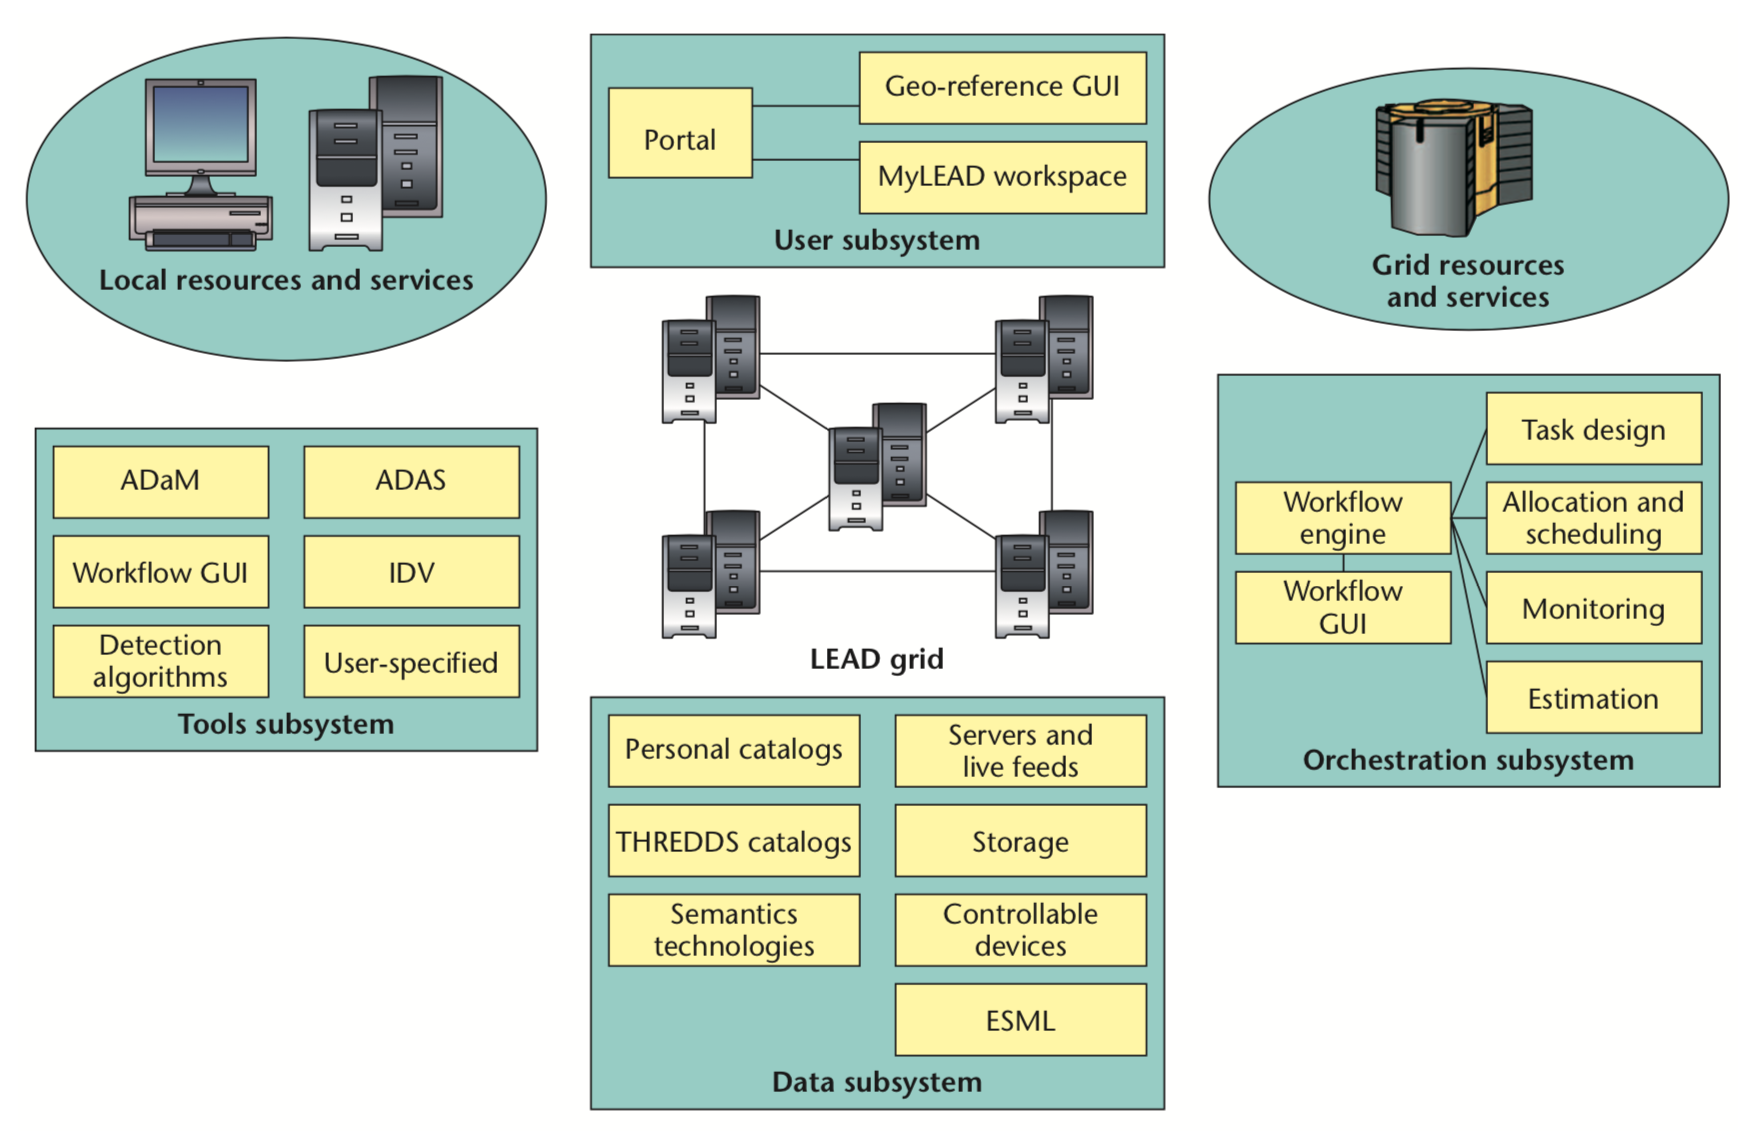
\includegraphics[width=1.0\textwidth]{lit/lead/LEAD-system-framework-LEAD-is-composed-of-several-interacting-subsystems-with-the-LEAD_W640.png}
    \caption[LEAD system framework]{LEAD system framework \cite{Droegemeier2005Service-orientedWeather}.}
    \label{fi:lead_framework}
\end{figure}

As shown in \cref{fi:lead_framework}, LEAD consists of the following sub-components, as well as provides a distributed system for integrating and testing LEAD's components:
\begin{itemize}
    \item User subsystem – comprises the LEAD portal and enable user can access services
    \item Data subsystem – manages data and metadata, all output of digital models produced by operational or experimental models, and information generated by users
    \item Tools subsystem – provides all IT tools and meteorological tools
    \item Orchestration subsystem – offers the technologies with which users can manage data flows and model execution flows and can create and own output
\end{itemize}

\begin{figure}[htp]
    \centering
    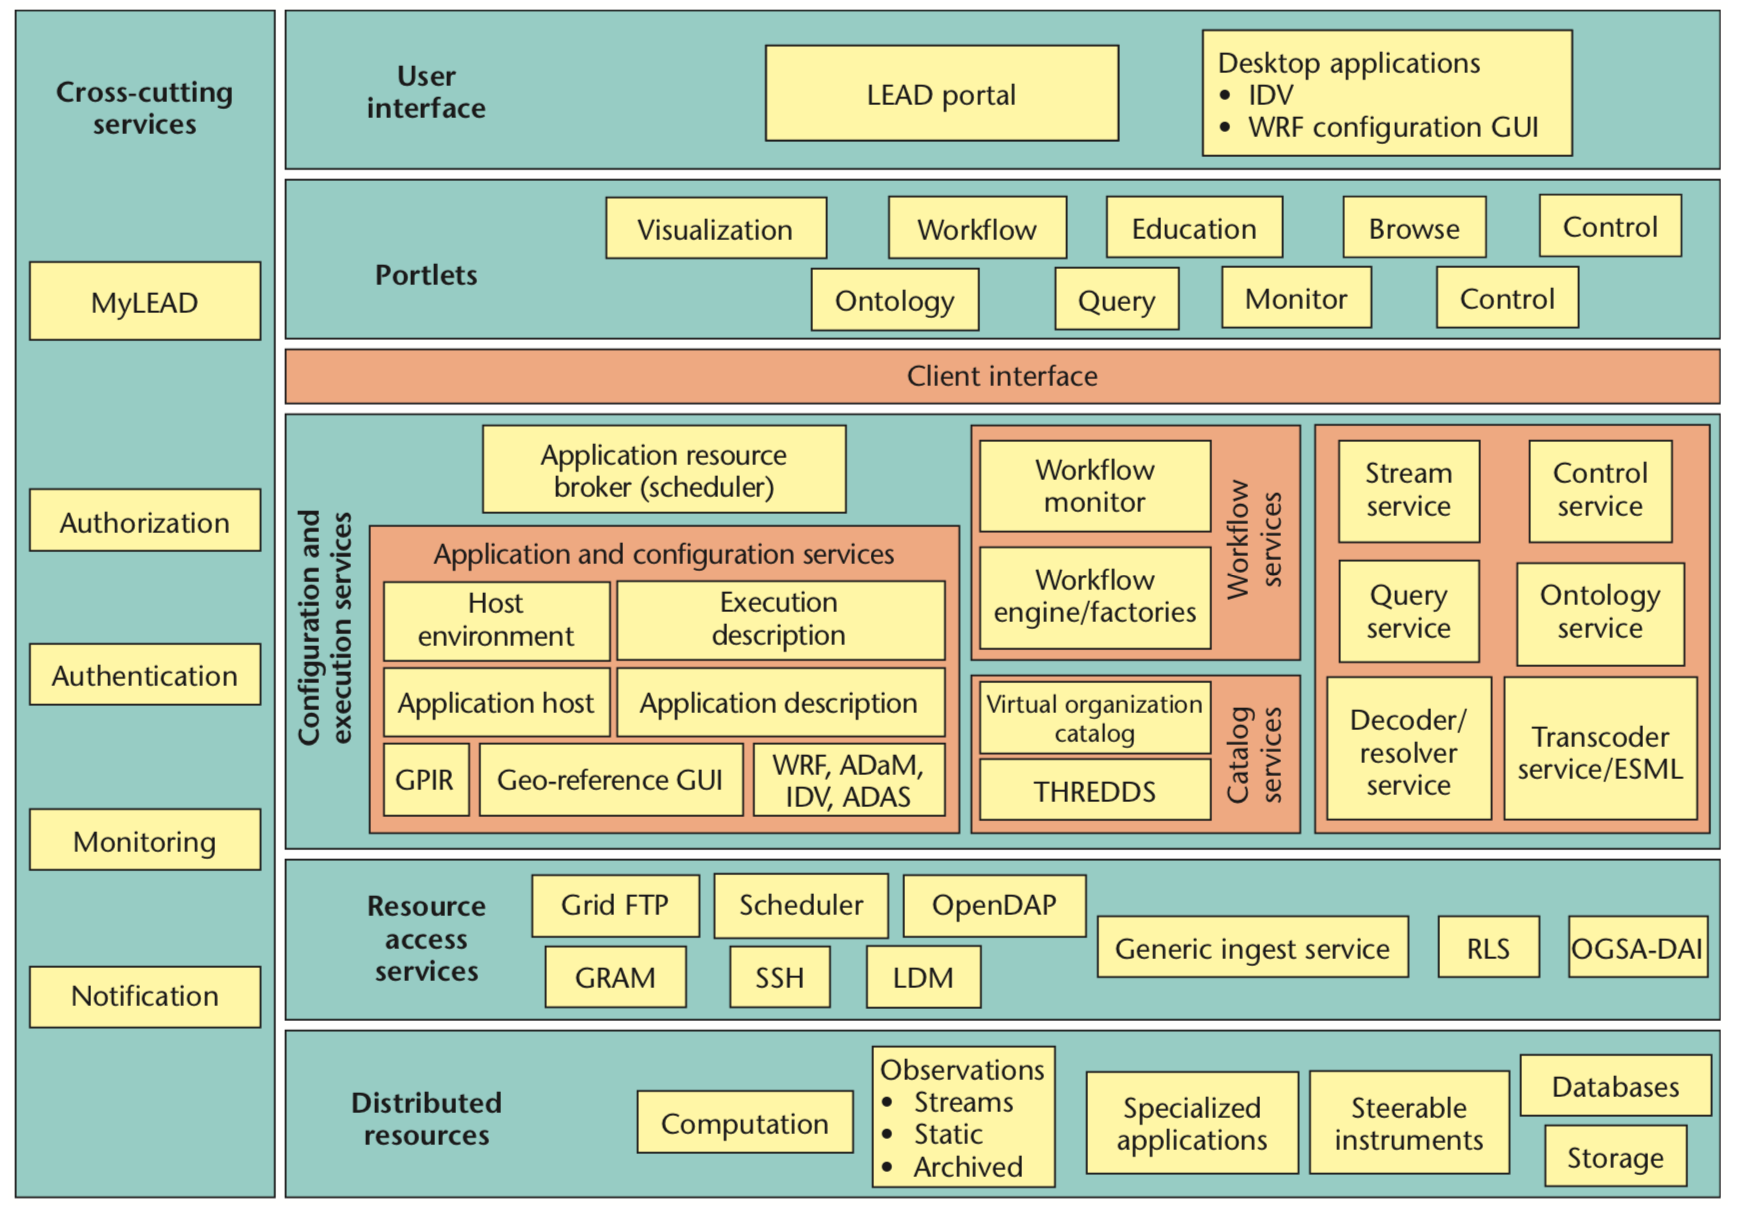
\includegraphics[width=1\textwidth]{lit/lead/LEADs-service-oriented-architecture-A-wide-variety-of-services-and-resources-grouped_W640.png}
    \caption[LEAD's service-oriented architecture]{LEAD's service-oriented architecture \cite{Droegemeier2005Service-orientedWeather}.}
    \label{fi:lead_soa}
\end{figure}

As shown in \cref{fi:lead_soa}, \acrshort{lead} \acrshort{soa} has five different but highly interconnected layers. The bottom layer represents the calculation, application, and raw data sources that are distributed in the LEAD grid and elsewhere. The next level supports web services that provide access to raw services \cite{Droegemeier2005Service-orientedWeather}. These two layers are working together since LEAD system resources are distributed over multiple locations and creating a pool of resources. The upper layer of the raw resources is abstracting the complexity of managing and accessing the resources and provides simplified access. In the upper layers, the underline system is viewed as an unlimited resource pool for storing and handling data.

The configuration and execution services of the middle layer, consisting of five elements, represent the services that call LEAD workflows. These are some critical aspects of a weather data management system. Most of the services listed below are required for creating workflows for weather data forecasting. While analyzing the LEAD, we realized that it is essential to understand the following basic needs of a weather data management system.

\begin{itemize}
    \item The application-oriented configuration service manages the implementation and execution of real applications, such as the WRF simulation model, ADAS, and ADaM tools [5]. While creating weather forecast workflows, the researchers require to change the behavior of the model by changing some of the configurations of the model or run a different version of the model.
    \item The application resource broker, which matches the appropriate host for execution to each application task, based on the execution time constraints [5]. This service is a critical part of the LEAD system and responsible for using the resource pool in an optimized manner. One important fact is, while we are designing weather data systems, it is required to increase the capacity of the system automatically, and manage the system.
    \item The workflow engine service, which manages the experimental workflow instances, invokes both the configuration service and the application resource broker [5]. The above service is a part of workflow orchestration.
    \item Catalog services represent how a user or an application service discovers data products in the public domain or LEAD services [5]. Most systems need a catalog service and essential to have such features because users need to search for the availability of the data, and users want to analyze existing data for decision making.
    \item Users need a multitude of data services to support comprehensive query, access, and transformation operations on data products. An essential goal behind LEAD is the transparency of access that facilitates user requests on all available heterogeneous data sources without the negative effects of different formats and naming schemes [5]. Users need to have transformation services to read data in different formats. The query service gives the capability to search via available data without any effect on the data formats.
\end{itemize}

The top of \cref{fi:lead_soa} shows the user interface of the LEAD, and each user gets individual access to services via the interface. After the user login into the system, the LEAD system allows portlets to access the services on half of the users based on the authentication and authorization setting of the account.

LEAD is a more advanced system which can support mesoscale weather forecast with the effort of multiple universities in the United State America with the effort of many researchers and using many computer resources. At the time of  building, it uses the \acrshort{soa} architecture into its depth, and at the implementation, each service can scale as needed and possible to enhance the service without interrupting other services. However, during our research, we only focus on creating a framework that is extendable as a system needs more features similar to LEAD services. When compared to the \acrshort{fews}, the \acrshort{lead} is more dynamic and auto scaling system which is capable of using a distributed large resource pool. But it is a proprietary system, thus others cannot get benefit of it, and the user need to own the resource pool and manage them. In critical situations the system need more resource for the forecasts, and users need to pre-owned the resources to get ready for such scenarios. But with modern cloud computing concepts, users can lease much as resources to handle the critical situation, and release the resource after that while only paying for the utilized resource duration.
